\documentclass{article}
\usepackage{graphicx}
\usepackage{subfigure}
\usepackage{multirow}
\usepackage{wrapfig}
\usepackage{amssymb}
\usepackage{amsfonts, amsmath}
\usepackage{amsmath}
\usepackage{mathrsfs}
\usepackage{enumerate}
% \usepackage[bookmarks=true]{hyperref}
% \usepackage[acronym]{glossaries}
%\usepackage{bookmark}
\usepackage{amssymb,amsmath,amsthm,amsfonts}
\usepackage{mathrsfs}
\usepackage{dsfont}
\usepackage{enumerate}

%\newtheorem{mdef}{Definition}
%\newtheorem{theorem}{Theorem}
\newcommand{\eqsplit}[2]{
  \begin{equation}\label{#2}
    \begin{split}
      #1
    \end{split}
  \end{equation}}
\newcommand{\eqnsplit}[1]{
  \begin{eqnarray*}
    #1
  \end{eqnarray*}}
\newcommand{\tran}[1]{
  \tilde{#1}
}
\newcommand{\td}[2]{
  \frac{d #1}{d #2}
}
\newcommand{\pd}[2]{
  \frac{\partial #1}{\partial #2}
}
\newcommand{\ppd}[2]{
  \frac{\partial^2 #1}{\partial #2^2}
}
\newcommand{\pdd}[3]{
  \frac{\partial^2 #1}{\partial #2 \partial #3}
}
\newcommand{\otd}[1]{
  \frac{d}{d #1}
}
\newcommand{\opd}[1]{
  \frac{\partial}{\partial #1}
}
\newcommand{\oppd}[1]{
  \frac{\partial^2}{\partial #1^2}
}
\newcommand{\opdd}[2]{
  \frac{\partial^2}{\partial #1 \partial #2}
}
\newcommand{\ket}[1]{
  |#1\rangle
}
\newcommand{\bra}[1]{
  \langle#1|
}
\newcommand{\inn}[1]{
  \langle#1\rangle
}
\newcommand{\mean}[1]{
  \langle#1\rangle
}
\newcommand{\tr}{
  \text{tr}\,
}
\newcommand{\re}{
  \text{Re}\,
}
\newcommand\im{
  \text{Im}\,
}
\newcommand{\var}{
  \text{var}
}
\newcommand{\arcsinh}{
  \sinh^{-1}
}
\newcommand{\arccosh}{
  \cosh^{-1}
}
\newcommand{\erfc}{
  \text{erfc}
}
\newcommand{\E}{
  \mathbb{E}
}
\renewcommand{\P}{
  \mathbb{P}
}
\newcommand{\I}[1]{
  \mathbf{1}_{\{#1\}}
}
\newcommand{\1}[1]{
  \mathds{1}_{\{#1\}}
}
\newcommand{\diag}{
  \text{diag\,}
}
\newcommand{\M}{
  {\text{max}}
}
\newcommand{\m}{
  {\text{min}}
}
\newcommand{\ph}{
  {\text{arg}\,}
}
\newcommand\erf{
  \text{erf}
}
\renewcommand\vec[1]{
  \mathbf{#1}
}
\newcommand\mtx[1]{
  \mathbf{#1}
}
\newcommand\ed{
  \,{\buildrel d \over =}\,
}




\DeclareGraphicsExtensions{.eps}

\begin{document}
\section{Distance to the MP law}
\begin{figure}[htb!]
  \centering
    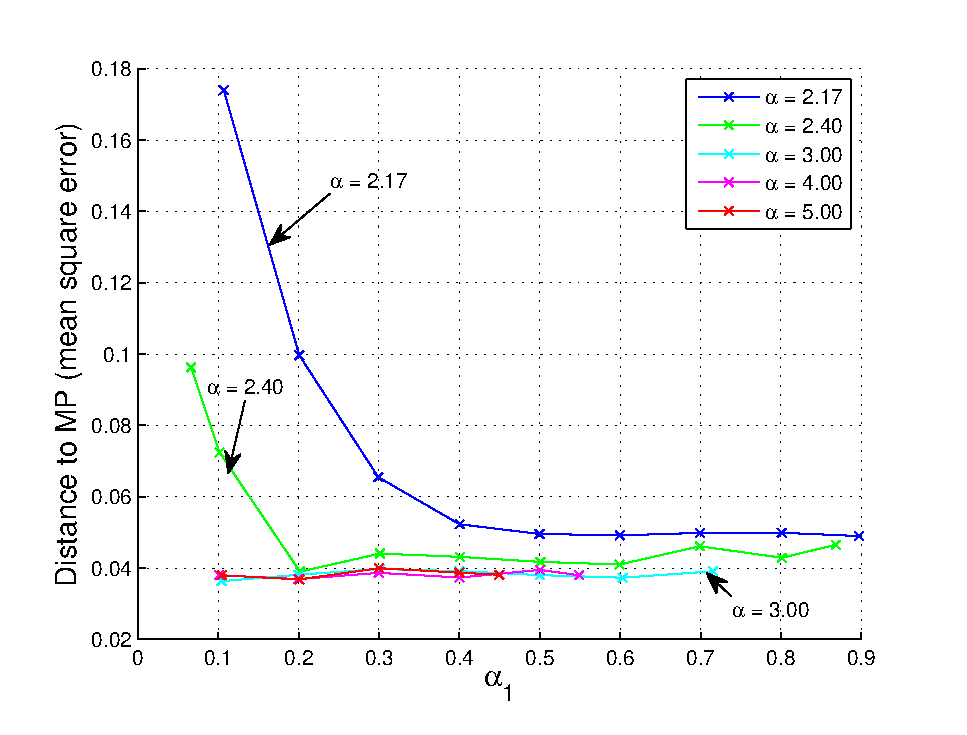
\includegraphics[scale=0.6]{../pics/Distance_to_MP.eps}
    \caption{\small \it Distance of the empirical spectral density to
      the Marchenko-Pastur law measured in terms of the mean square
      error between the two density functions}
    \label{fig:Distance_to_MP}
\end{figure}

\section{Spectral Density with Fixed $\alpha_1$}
% \begin{figure}[htb!]
%   \centering
%   \subfigure[Spectral density with $\alpha_1$ fixed to 0.1
%   and the tail expoent $\alpha$ varying.] {
%     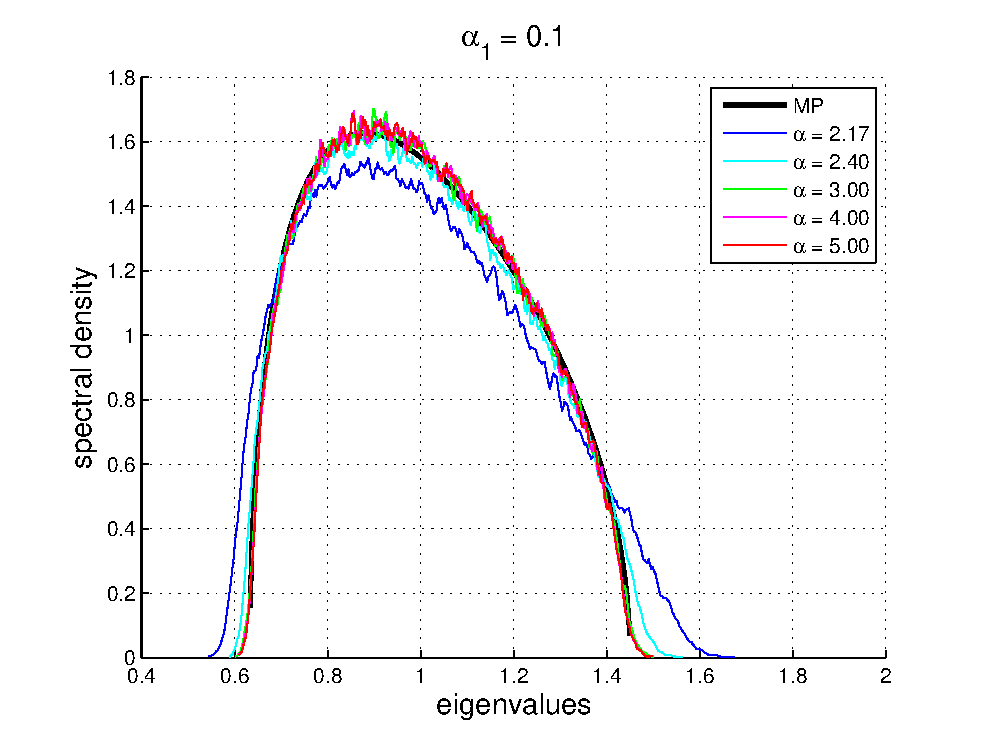
\includegraphics[scale=0.35]{../pics/Spectral_density_fixed_alpha1_0.1.eps}
%     \label{fig:spectral_density_fixed_alpha1_0.1}
%   }
%   \subfigure[Largest eigenvalue distribution with $\alpha_1$ fixed to 0.1
%   and the tail expoent $\alpha$ varying.] {
%     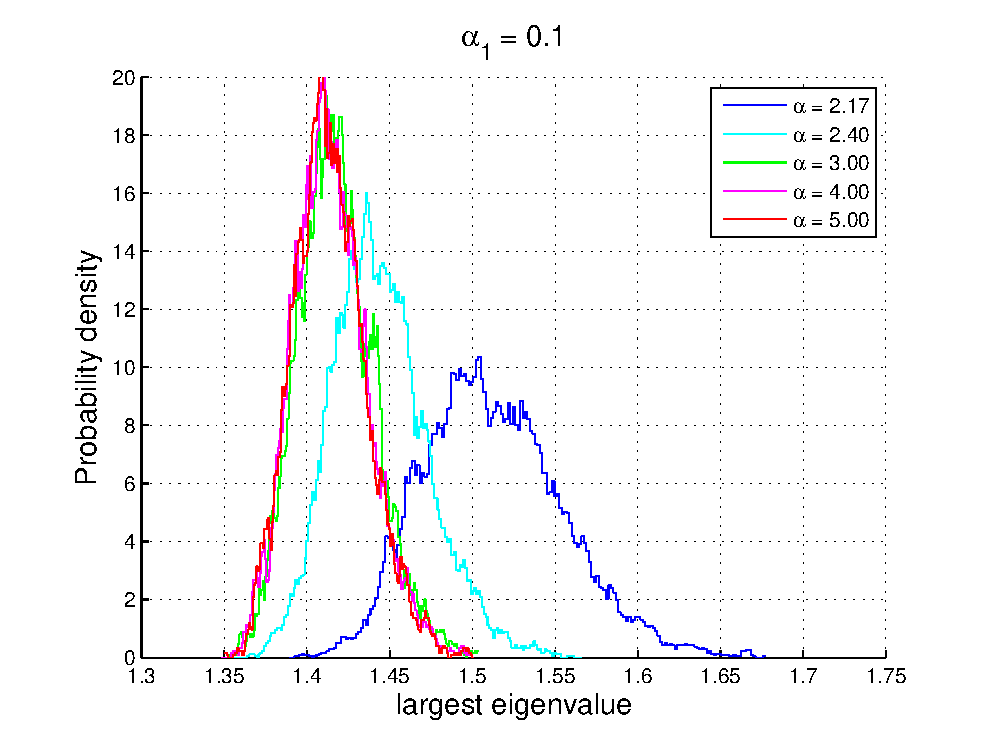
\includegraphics[scale=0.35]{../pics/eigmax_dist_fixed_alpha1_0.1.eps}
%     \label{fig:eigmax_dist_fixed_alpha1_0.1}
%   }

%   \subfigure[Spectral density with $\alpha_1$ fixed to 0.2
%   and the tail expoent $\alpha$ varying.] {
%     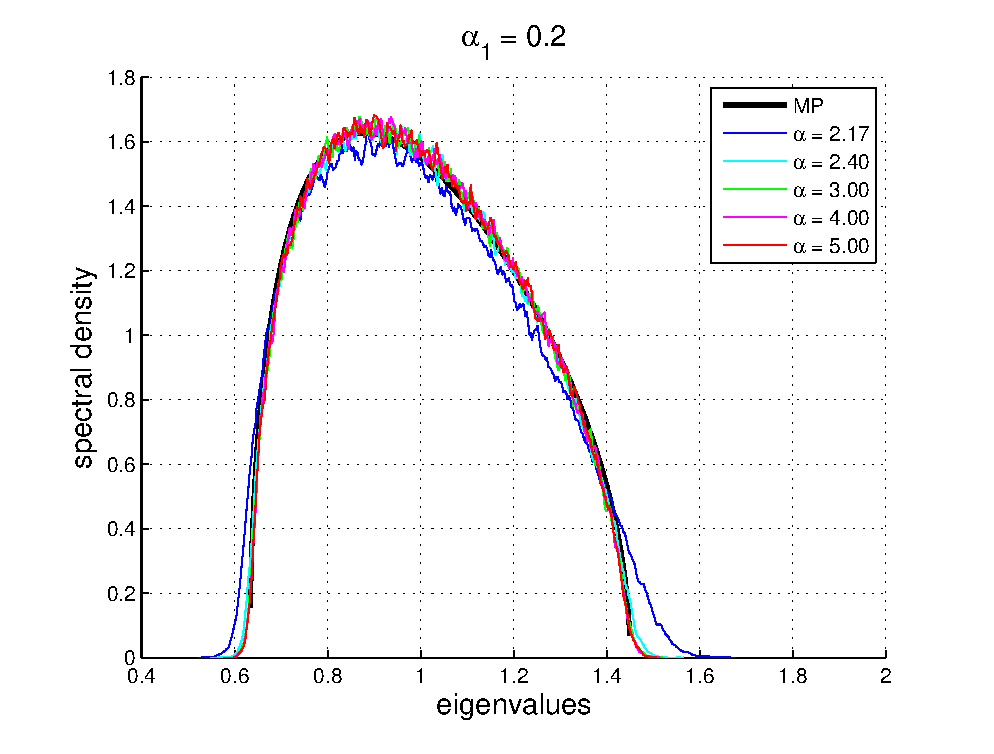
\includegraphics[scale=0.35]{../pics/Spectral_density_fixed_alpha1_0.2.eps}
%     \label{fig:spectral_density_fixed_alpha1_0.2}
%   }
%   \subfigure[Largest eigenvalue distribution with $\alpha_1$ fixed to 0.2
%   and the tail expoent $\alpha$ varying.] {
%     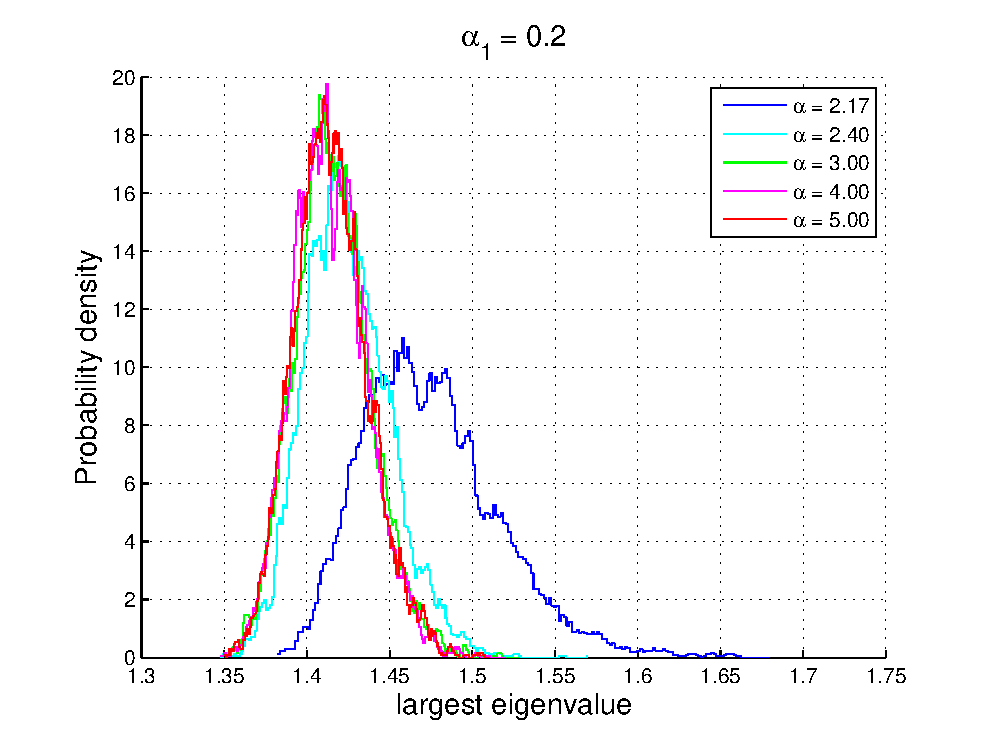
\includegraphics[scale=0.35]{../pics/eigmax_dist_fixed_alpha1_0.2.eps}
%     \label{fig:eigmax_dist_fixed_alpha1_0.2}
%   }

%   \subfigure[Spectral density with $\alpha_1$ fixed to 0.3
%   and the tail expoent $\alpha$ varying.] {
%     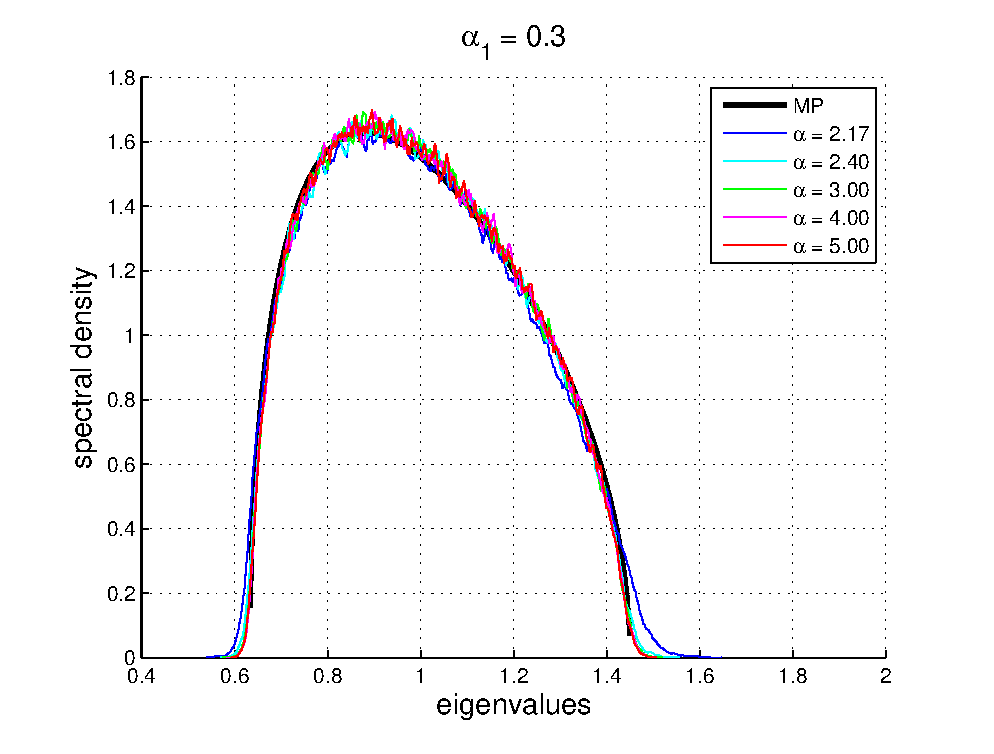
\includegraphics[scale=0.35]{../pics/Spectral_density_fixed_alpha1_0.3.eps}
%     \label{fig:spectral_density_fixed_alpha1_0.3}
%   }
%   \subfigure[Largest eigenvalue distribution with $\alpha_1$ fixed to 0.3
%   and the tail expoent $\alpha$ varying.] {
%     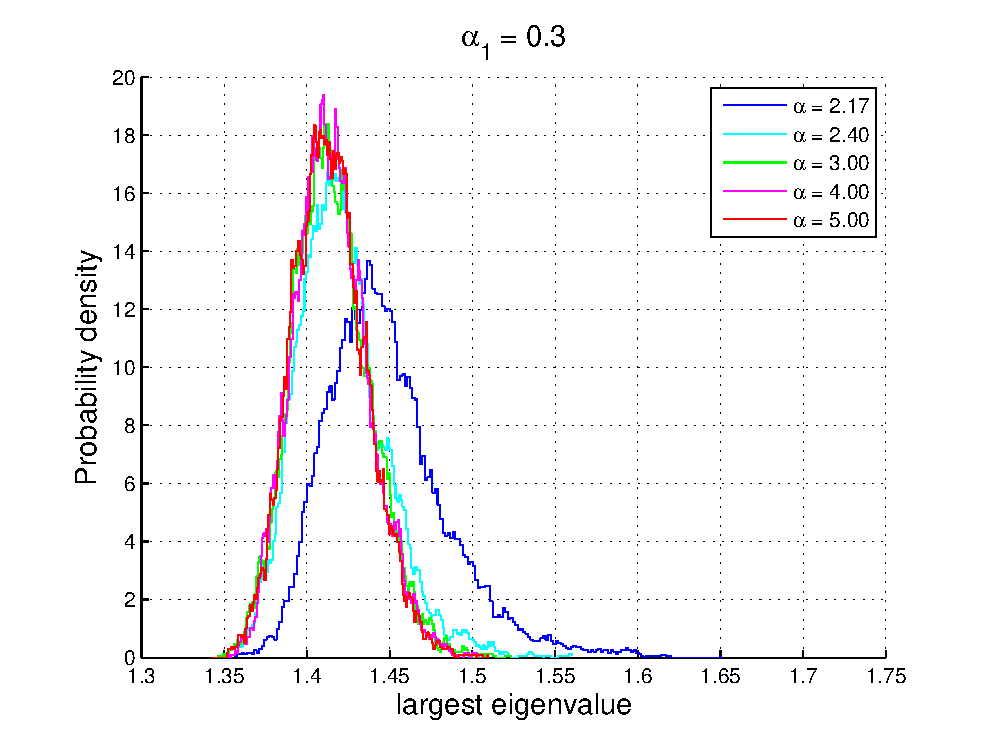
\includegraphics[scale=0.35]{../pics/eigmax_dist_fixed_alpha1_0.3.eps}
%     \label{fig:eigmax_dist_fixed_alpha1_0.3}
%   }
%   \caption{Spectral Density with Fixed $\alpha_1$}
%   \label{fig:spectral_density_fixed_alpha1}
% \end{figure}

\begin{figure}[htb!]
  \centering
  \subfigure[Spectral density with $\alpha_1$ fixed to 0.1
  and the tail expoent $\alpha$ varying.] {
    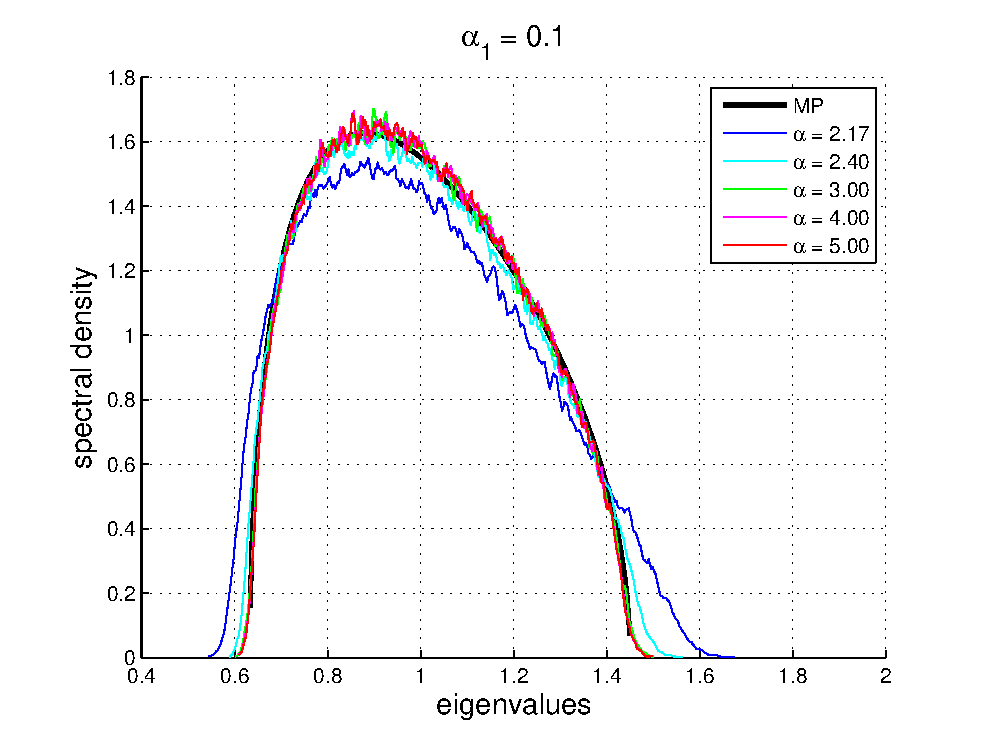
\includegraphics[scale=0.35]{../pics/Spectral_density_fixed_alpha1_0.1.eps}
    \label{fig:spectral_density_fixed_alpha1_0.1}
  }
  \subfigure[Smallest eigenvalue distribution with $\alpha_1$ fixed to 0.1
  and the tail expoent $\alpha$ varying.] {
    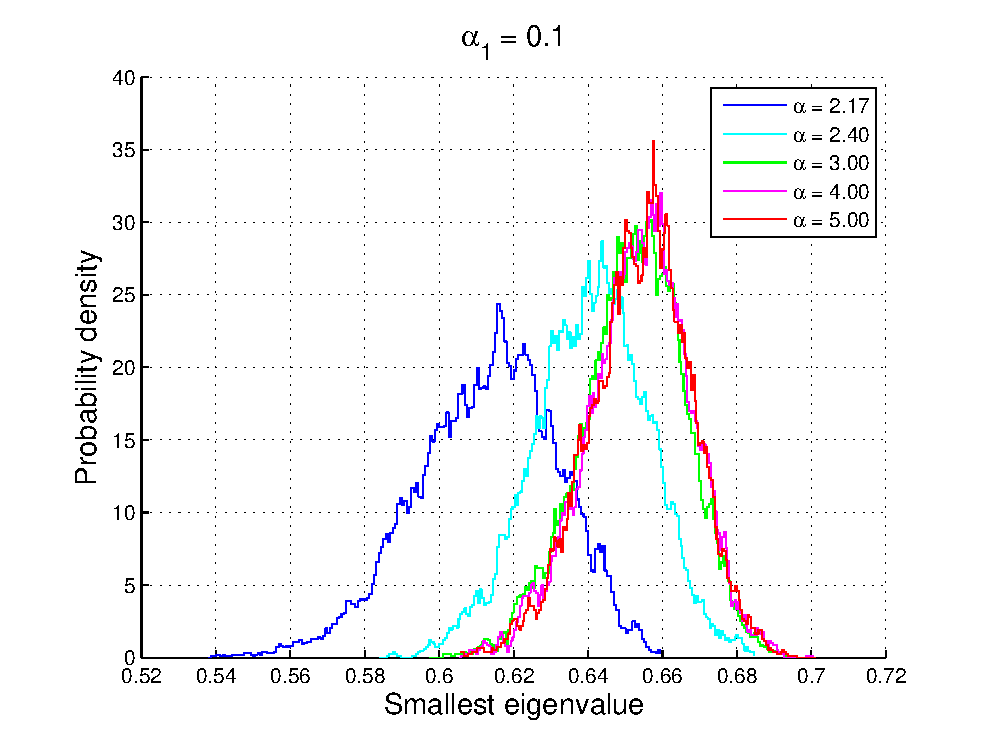
\includegraphics[scale=0.35]{../pics/eigmin_dist_fixed_alpha1_0.1.eps}
    \label{fig:eigmin_dist_fixed_alpha1_0.1}
  }
  \subfigure[Spectral density with $\alpha_1$ fixed to 0.2
  and the tail expoent $\alpha$ varying.] {
    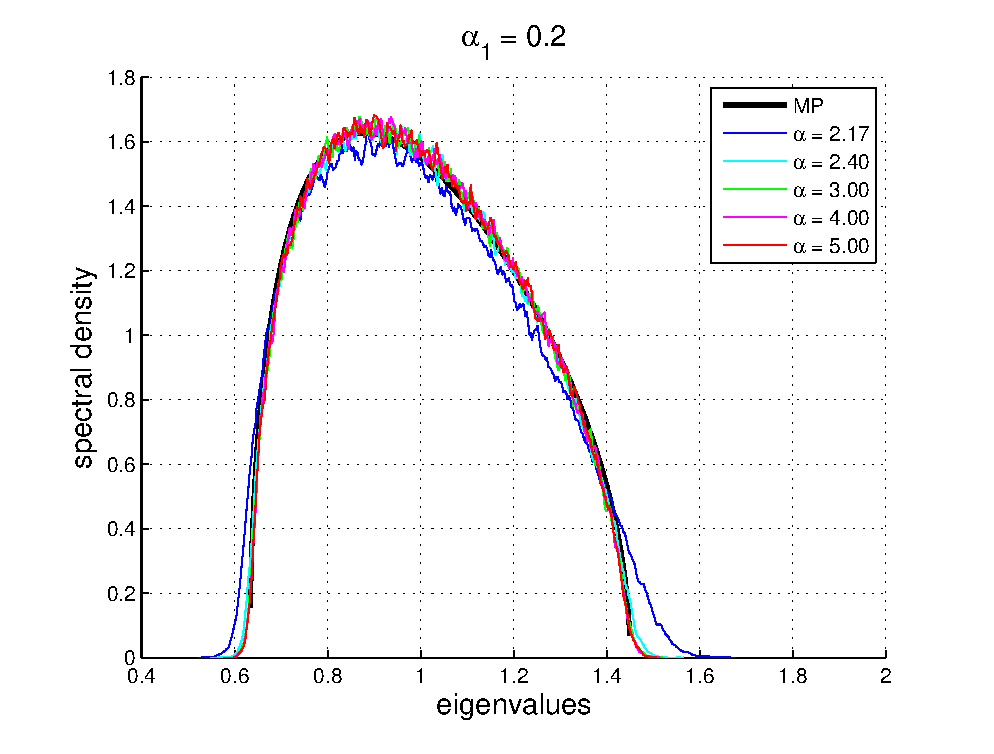
\includegraphics[scale=0.35]{../pics/Spectral_density_fixed_alpha1_0.2.eps}
    \label{fig:spectral_density_fixed_alpha1_0.2}
  }
  \subfigure[Smallest eigenvalue distribution with $\alpha_1$ fixed to 0.2
  and the tail expoent $\alpha$ varying.] {
    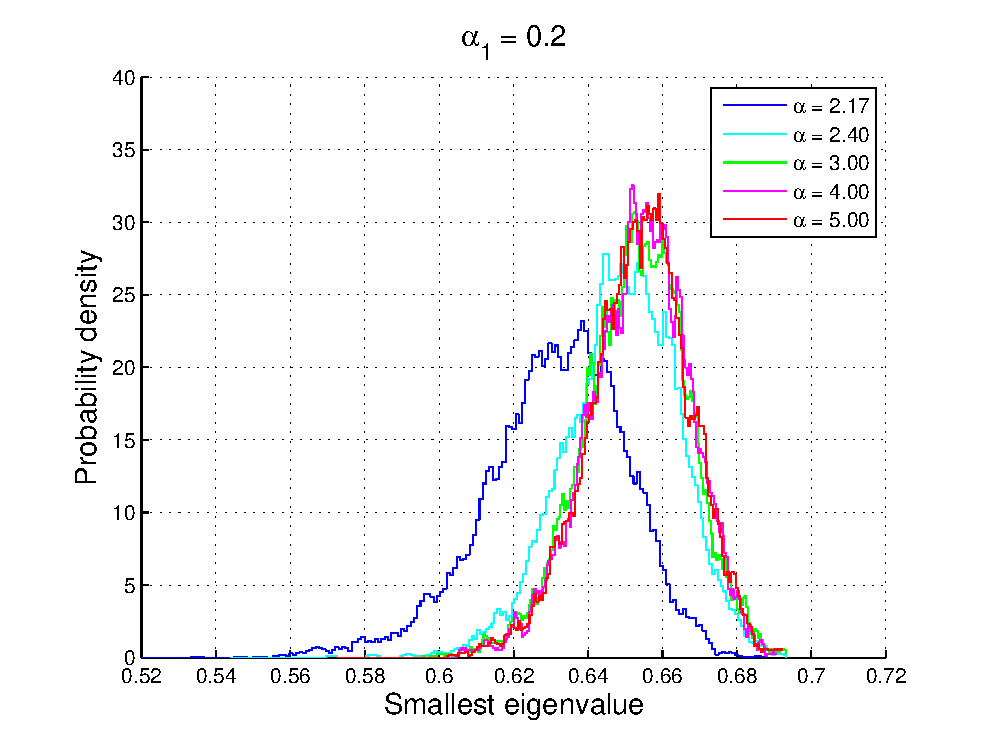
\includegraphics[scale=0.35]{../pics/eigmin_dist_fixed_alpha1_0.2.eps}
    \label{fig:eigmin_dist_fixed_alpha1_0.2}
  }

  \subfigure[Spectral density with $\alpha_1$ fixed to 0.3
  and the tail expoent $\alpha$ varying.] {
    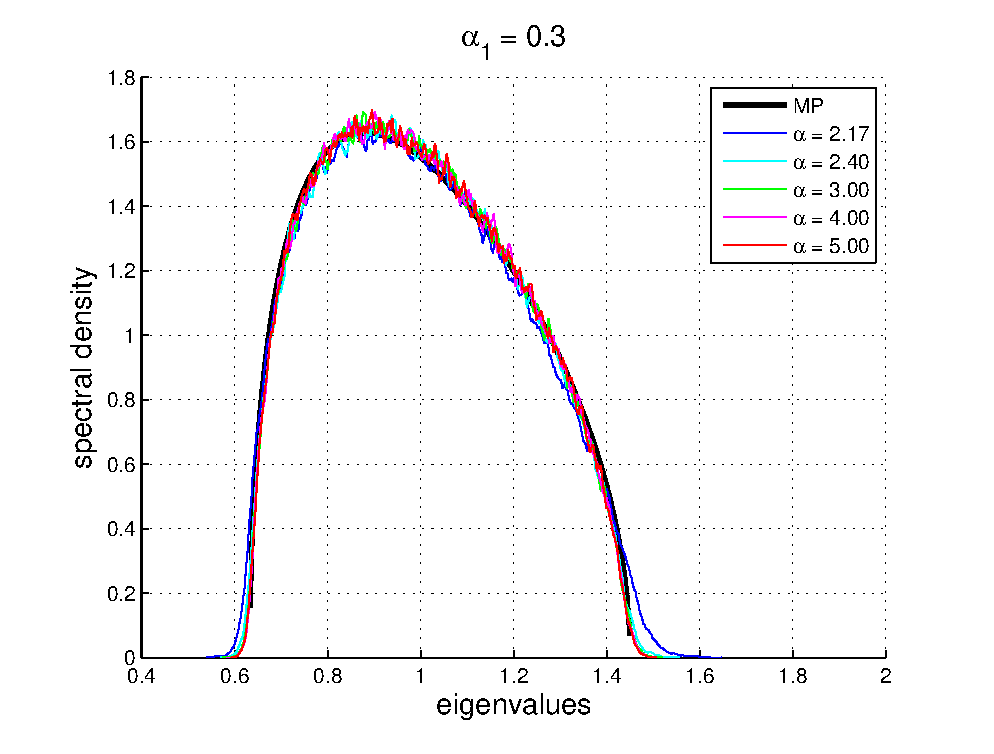
\includegraphics[scale=0.35]{../pics/Spectral_density_fixed_alpha1_0.3.eps}
    \label{fig:spectral_density_fixed_alpha1_0.3}
  }
  \subfigure[Smallest eigenvalue distribution with $\alpha_1$ fixed to 0.3
  and the tail expoent $\alpha$ varying.] {
    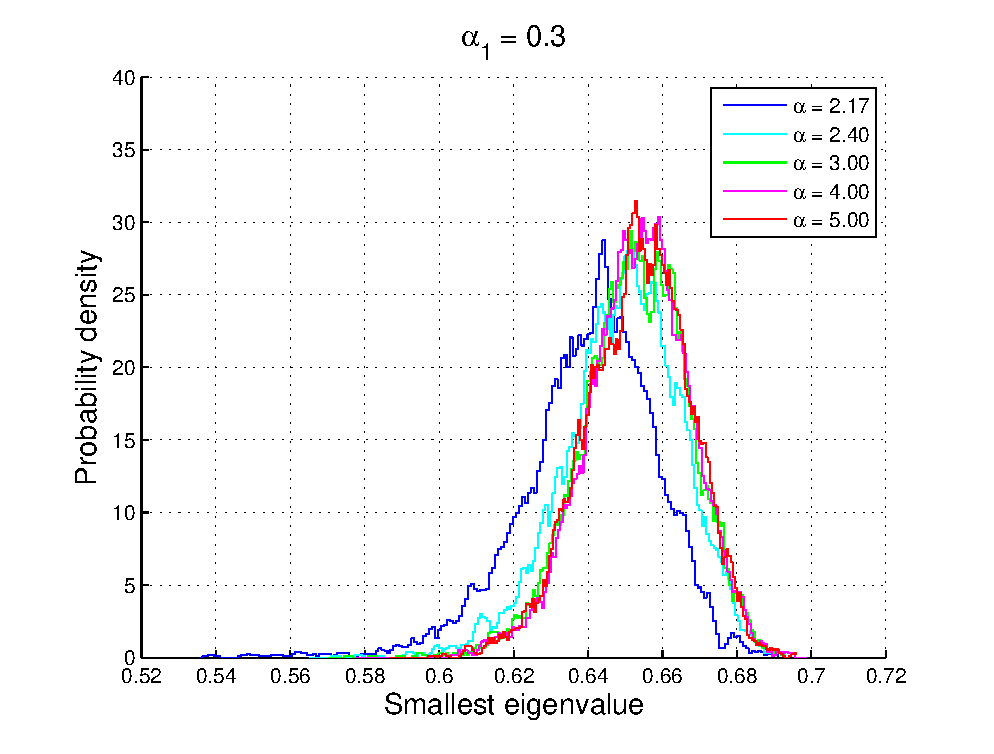
\includegraphics[scale=0.35]{../pics/eigmin_dist_fixed_alpha1_0.3.eps}
    \label{fig:eigmin_dist_fixed_alpha1_0.3}
  }
  \caption{Spectral Density with Fixed $\alpha_1$}
  \label{fig:spectral_density_fixed_alpha1}
\end{figure}

\end{document}